% \documentclass{article}
% \usepackage{amsmath}
% \usepackage{graphicx}
% \usepackage[margin=2cm]{geometry}
% \title{Modified Coin-Collecting Problem}
% \author{}
% \date{}
% \begin{document}
% \maketitle
% \section{Algorithm Description}
% Given a board with coins and barriers, the algorithm computes the maximum number of coins collectible and the path to collect them. Let \( F(i, j) \) represent the maximum number of coins collectible at cell \((i, j)\). The transition is modified to account for barriers:
% \[ 
% F(i, j) = 
% \begin{cases} 
% -1 & \text{if } B[i, j] = 1 \\ 
% \max(F(i-1, j), F(i, j-1)) + C[i, j] & \text{otherwise}\\
% F(0,j)=0 & \text{for } 1 \leq j \leq m\\
% F(i,0)=0 & \text{for } 1 \leq i \leq n
% \end{cases}
% \]
% This is the same as the algorithm in textbook, except where \( B[i, j] = 1 \) indicates an inaccessible cell.

% \section{Pseudocode}
% \begin{verbatim}
% ModifiedCoinCollection(C[1..n, 1..m], B[1..n, 1..m])
% if B[1, 1] = 1 or B[n, m] = 1 then return 0
% F[1, 1] = C[1, 1]
% for j = 2 to m do
%     if B[1, j] = 0 then F[1, j] = F[1, j-1] + C[1, j]
%     else F[1, j] = -1
% for i = 2 to n do
%     if B[i, 1] = 0 then F[i, 1] = F[i-1, 1] + C[i, 1]
%     else F[i, 1] = -1
% for i = 2 to n do
%     for j = 2 to m do
%         if B[i, j] = 0 then F[i, j] = max(F[i-1, j], F[i, j-1]) + C[i, j]
%         else F[i, j] = -1
% return max(F[n, m], 0)
% \end{verbatim}

% \section{Problem Instances}
% Ignoring the ties, The solutions to the problem instances are as follows:

% \end{document}
\documentclass{article}
\usepackage{amsmath}
\usepackage{graphicx}

\title{Homework 6 Solutions}
\author{}
\date{}

\begin{document}

\maketitle

\section{Problem 1: Explanation of the Modified Algorithm}
The modified algorithm introduces barriers (inaccessible cells) on the board. This means that the robot cannot move through these cells. To handle this, we modify the dynamic programming formula to account for barriers. Specifically, if a cell (i, j) is inaccessible, the value of $F(i, j)$ is set to $-\infty$ (or a very negative number) to indicate that this cell cannot be part of the path. The new formula becomes:

\[
F(i, j) = 
\begin{cases} 
-1 & \text{if } B(i, j) = 1 \\
\max(F(i-1, j), F(i, j-1)) + c_{ij} & \text{otherwise}
\end{cases}
\]

\section{Problem 2: Pseudocode for the Modified Algorithm}
\subsection{Pseudocode}
The algorithm marks the first cell of the f matrix with the value of the first cell of the c matrix. Then, it fills the first row and column of the f matrix with the sum of the previous cell and the current cell if the current cell is accessible. 
Otherwise, it marks the cell as inaccessible. 
terate through the remaining cells. For each cell:
If the cell is not blocked, check the cells above and to the left. If both cells have valid paths, take the maximum of the two values and add the current cell's coin value.
If only one of the cells (either above or left) has a valid path, use that value.
If neither cell has a valid path, set the current cell to -1.
If the cell is blocked, set it to -1.
The algorithm returns the maximum value in the last cell of the f matrix.
\begin{verbatim}
ModifiedCoinCollection(C[1..n, 1..m], B[1..n, 1..m])
    if B[1, 1] = 1 or B[n, m] = 1 then return 0
    
    F[1, 1] = C[1, 1]
    
    for j = 2 to m do
        if B[1, j] = 0 and F[1, j-1] != -1 then
            F[1, j] = F[1, j-1] + C[1, j]
        else
            F[1, j] = -1
    
    for i = 2 to n do
        if B[i, 1] = 0 and F[i-1, 1] != -1 then
            F[i, 1] = F[i-1, 1] + C[i, 1]
        else
            F[i, 1] = -1
    
    for i = 2 to n do
        for j = 2 to m do
            if B[i, j] = 0 then
                if F[i-1, j] != -1 and F[i, j-1] != -1 then
                    F[i, j] = max(F[i-1, j], F[i, j-1]) + C[i, j]
                elif F[i-1, j] != -1 then
                    F[i, j] = F[i-1, j] + C[i, j]
                elif F[i, j-1] != -1 then
                    F[i, j] = F[i, j-1] + C[i, j]
                else
                    F[i, j] = -1
            else
                F[i, j] = -1
    
    return max(F[n, m], 0)
\end{verbatim}

\section{Problem 3: Solve the Given Problem Instances}
Let's compute the matrix $F$ for each of the given problem instances.
\subsection{Instance 1}
\subsubsection{Filling the $F$ Matrix}
\begin{figure}[!h]
    \centering
    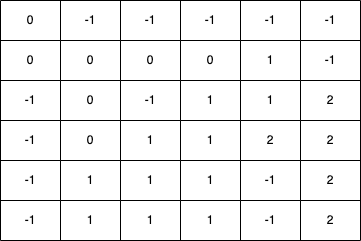
\includegraphics[width=0.5\textwidth]{image.png}
    \caption{optimal paths shown with a line}
    \label{fig:instance1}
\end{figure}

The maximum number of coins collectible is 2. fig~\ref{fig:instance1}

\subsection{Instance 2}
\subsubsection{Filling the $F$ Matrix}
\begin{figure}[!h]
    \centering
    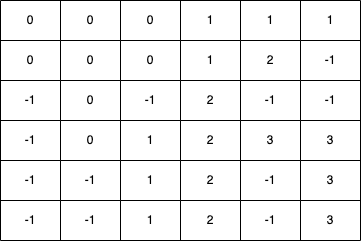
\includegraphics[width=0.5\textwidth]{image2.png}
    \caption{optimal paths shown with a line}
    \label{fig:instance2}
\end{figure}

The maximum number of coins collectible is 3. fig~\ref{fig:instance2}

\subsection{Instance 3}
\subsubsection{Filling the $F$ Matrix}
\begin{figure}[!h]
    \centering
    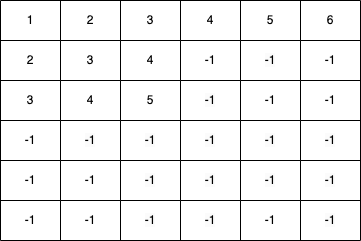
\includegraphics[width=0.5\textwidth]{image3.png}
    \caption{optimal paths shown with a line}
    \label{fig:instance3}
\end{figure}
The maximum number of coins collectible is 0. fig~\ref{fig:instance3}
\end{document}
